\documentclass[twoside]{book}

% Packages required by doxygen
\usepackage{fixltx2e}
\usepackage{calc}
\usepackage{doxygen}
\usepackage[export]{adjustbox} % also loads graphicx
\usepackage{graphicx}
\usepackage[utf8]{inputenc}
\usepackage{makeidx}
\usepackage{multicol}
\usepackage{multirow}
\PassOptionsToPackage{warn}{textcomp}
\usepackage{textcomp}
\usepackage[nointegrals]{wasysym}
\usepackage[table]{xcolor}

% Font selection
\usepackage[T1]{fontenc}
\usepackage[scaled=.90]{helvet}
\usepackage{courier}
\usepackage{amssymb}
\usepackage{sectsty}
\renewcommand{\familydefault}{\sfdefault}
\allsectionsfont{%
  \fontseries{bc}\selectfont%
  \color{darkgray}%
}
\renewcommand{\DoxyLabelFont}{%
  \fontseries{bc}\selectfont%
  \color{darkgray}%
}
\newcommand{\+}{\discretionary{\mbox{\scriptsize$\hookleftarrow$}}{}{}}

% Page & text layout
\usepackage{geometry}
\geometry{%
  a4paper,%
  top=2.5cm,%
  bottom=2.5cm,%
  left=2.5cm,%
  right=2.5cm%
}
\tolerance=750
\hfuzz=15pt
\hbadness=750
\setlength{\emergencystretch}{15pt}
\setlength{\parindent}{0cm}
\setlength{\parskip}{3ex plus 2ex minus 2ex}
\makeatletter
\renewcommand{\paragraph}{%
  \@startsection{paragraph}{4}{0ex}{-1.0ex}{1.0ex}{%
    \normalfont\normalsize\bfseries\SS@parafont%
  }%
}
\renewcommand{\subparagraph}{%
  \@startsection{subparagraph}{5}{0ex}{-1.0ex}{1.0ex}{%
    \normalfont\normalsize\bfseries\SS@subparafont%
  }%
}
\makeatother

% Headers & footers
\usepackage{fancyhdr}
\pagestyle{fancyplain}
\fancyhead[LE]{\fancyplain{}{\bfseries\thepage}}
\fancyhead[CE]{\fancyplain{}{}}
\fancyhead[RE]{\fancyplain{}{\bfseries\leftmark}}
\fancyhead[LO]{\fancyplain{}{\bfseries\rightmark}}
\fancyhead[CO]{\fancyplain{}{}}
\fancyhead[RO]{\fancyplain{}{\bfseries\thepage}}
\fancyfoot[LE]{\fancyplain{}{}}
\fancyfoot[CE]{\fancyplain{}{}}
\fancyfoot[RE]{\fancyplain{}{\bfseries\scriptsize Generated by Doxygen }}
\fancyfoot[LO]{\fancyplain{}{\bfseries\scriptsize Generated by Doxygen }}
\fancyfoot[CO]{\fancyplain{}{}}
\fancyfoot[RO]{\fancyplain{}{}}
\renewcommand{\footrulewidth}{0.4pt}
\renewcommand{\chaptermark}[1]{%
  \markboth{#1}{}%
}
\renewcommand{\sectionmark}[1]{%
  \markright{\thesection\ #1}%
}

% Indices & bibliography
\usepackage{natbib}
\usepackage[titles]{tocloft}
\setcounter{tocdepth}{3}
\setcounter{secnumdepth}{5}
\makeindex

% Hyperlinks (required, but should be loaded last)
\usepackage{ifpdf}
\ifpdf
  \usepackage[pdftex,pagebackref=true]{hyperref}
\else
  \usepackage[ps2pdf,pagebackref=true]{hyperref}
\fi
\hypersetup{%
  colorlinks=true,%
  linkcolor=blue,%
  citecolor=blue,%
  unicode%
}

% Custom commands
\newcommand{\clearemptydoublepage}{%
  \newpage{\pagestyle{empty}\cleardoublepage}%
}

\usepackage{caption}
\captionsetup{labelsep=space,justification=centering,font={bf},singlelinecheck=off,skip=4pt,position=top}

%===== C O N T E N T S =====

\begin{document}

% Titlepage & ToC
\hypersetup{pageanchor=false,
             bookmarksnumbered=true,
             pdfencoding=unicode
            }
\pagenumbering{alph}
\begin{titlepage}
\vspace*{7cm}
\begin{center}%
{\Large Grim\+Engine }\\
\vspace*{1cm}
{\large Generated by Doxygen 1.8.14}\\
\end{center}
\end{titlepage}
\clearemptydoublepage
\pagenumbering{roman}
\tableofcontents
\clearemptydoublepage
\pagenumbering{arabic}
\hypersetup{pageanchor=true}

%--- Begin generated contents ---
\chapter{L\+I\+C\+E\+N\+SE}
\label{md__l_i_c_e_n_s_e}
\Hypertarget{md__l_i_c_e_n_s_e}
The M\+IT License (M\+IT)

Copyright (c) 2018 Ramon Meza

Permission is hereby granted, free of charge, to any person obtaining a copy of this software and associated documentation files (the \char`\"{}\+Software\char`\"{}), to deal in the Software without restriction, including without limitation the rights to use, copy, modify, merge, publish, distribute, sublicense, and/or sell copies of the Software, and to permit persons to whom the Software is furnished to do so, subject to the following conditions\+:

The above copyright notice and this permission notice shall be included in all copies or substantial portions of the Software.

T\+HE S\+O\+F\+T\+W\+A\+RE IS P\+R\+O\+V\+I\+D\+ED \char`\"{}\+A\+S I\+S\char`\"{}, W\+I\+T\+H\+O\+UT W\+A\+R\+R\+A\+N\+TY OF A\+NY K\+I\+ND, E\+X\+P\+R\+E\+SS OR I\+M\+P\+L\+I\+ED, I\+N\+C\+L\+U\+D\+I\+NG B\+UT N\+OT L\+I\+M\+I\+T\+ED TO T\+HE W\+A\+R\+R\+A\+N\+T\+I\+ES OF M\+E\+R\+C\+H\+A\+N\+T\+A\+B\+I\+L\+I\+TY, F\+I\+T\+N\+E\+SS F\+OR A P\+A\+R\+T\+I\+C\+U\+L\+AR P\+U\+R\+P\+O\+SE A\+ND N\+O\+N\+I\+N\+F\+R\+I\+N\+G\+E\+M\+E\+NT. IN NO E\+V\+E\+NT S\+H\+A\+LL T\+HE A\+U\+T\+H\+O\+RS OR C\+O\+P\+Y\+R\+I\+G\+HT H\+O\+L\+D\+E\+RS BE L\+I\+A\+B\+LE F\+OR A\+NY C\+L\+A\+IM, D\+A\+M\+A\+G\+ES OR O\+T\+H\+ER L\+I\+A\+B\+I\+L\+I\+TY, W\+H\+E\+T\+H\+ER IN AN A\+C\+T\+I\+ON OF C\+O\+N\+T\+R\+A\+CT, T\+O\+RT OR O\+T\+H\+E\+R\+W\+I\+SE, A\+R\+I\+S\+I\+NG F\+R\+OM, O\+UT OF OR IN C\+O\+N\+N\+E\+C\+T\+I\+ON W\+I\+TH T\+HE S\+O\+F\+T\+W\+A\+RE OR T\+HE U\+SE OR O\+T\+H\+ER D\+E\+A\+L\+I\+N\+GS IN T\+HE S\+O\+F\+T\+W\+A\+RE. 
\chapter{Hierarchical Index}
\section{Class Hierarchy}
This inheritance list is sorted roughly, but not completely, alphabetically\+:\begin{DoxyCompactList}
\item Drawable\begin{DoxyCompactList}
\item \contentsline{section}{Character}{\pageref{class_character}}{}
\item \contentsline{section}{State}{\pageref{class_state}}{}
\end{DoxyCompactList}
\item \contentsline{section}{Engine}{\pageref{class_engine}}{}
\item \contentsline{section}{Input\+Manager}{\pageref{class_input_manager}}{}
\item \contentsline{section}{State\+Manager}{\pageref{class_state_manager}}{}
\end{DoxyCompactList}

\chapter{Class Index}
\section{Class List}
Here are the classes, structs, unions and interfaces with brief descriptions\+:\begin{DoxyCompactList}
\item\contentsline{section}{\mbox{\hyperlink{class_character}{Character}} \\*Class for generic characters }{\pageref{class_character}}{}
\item\contentsline{section}{\mbox{\hyperlink{class_engine}{Engine}} \\*Base class for the game being developed }{\pageref{class_engine}}{}
\item\contentsline{section}{\mbox{\hyperlink{class_input_manager}{Input\+Manager}} \\*Handles input bindings }{\pageref{class_input_manager}}{}
\item\contentsline{section}{\mbox{\hyperlink{class_state}{State}} \\*Base class for any screen in the game, including levels }{\pageref{class_state}}{}
\item\contentsline{section}{\mbox{\hyperlink{class_state_manager}{State\+Manager}} \\*Acts as a wrapper to std\+::stack }{\pageref{class_state_manager}}{}
\end{DoxyCompactList}

\chapter{Class Documentation}
\hypertarget{class_character}{}\section{Character Class Reference}
\label{class_character}\index{Character@{Character}}


Class for generic characters.  




{\ttfamily \#include $<$Character.\+hpp$>$}

Inheritance diagram for Character\+:\begin{figure}[H]
\begin{center}
\leavevmode
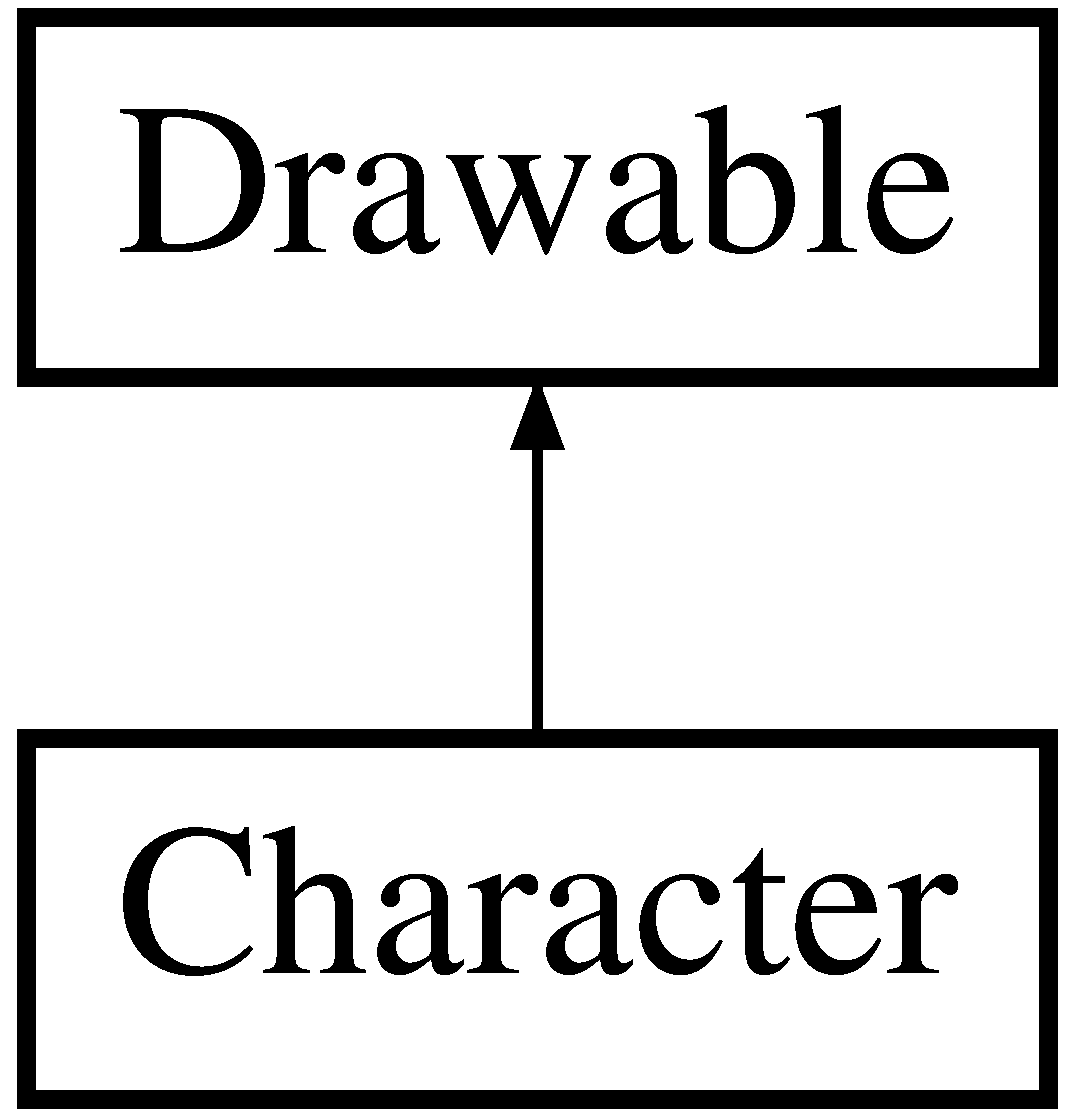
\includegraphics[height=2.000000cm]{class_character}
\end{center}
\end{figure}
\subsection*{Public Member Functions}
\begin{DoxyCompactItemize}
\item 
\mbox{\hyperlink{class_character_a9c0bcc7f37b218c920d014bf722037fa}{Character}} (std\+::string texture\+Path)
\begin{DoxyCompactList}\small\item\em Construct a character with the given texture path. \end{DoxyCompactList}\item 
\mbox{\Hypertarget{class_character_a9e9be564d05ded80962b2045aa70b3fc}\label{class_character_a9e9be564d05ded80962b2045aa70b3fc}} 
virtual \mbox{\hyperlink{class_character_a9e9be564d05ded80962b2045aa70b3fc}{$\sim$\+Character}} ()
\begin{DoxyCompactList}\small\item\em Virtual destructor. \end{DoxyCompactList}\item 
\mbox{\Hypertarget{class_character_a6e2226e97067453d9d4b131a8e0f9533}\label{class_character_a6e2226e97067453d9d4b131a8e0f9533}} 
{\footnotesize template$<$typename ... Args$>$ }\\void {\bfseries move} (Args \&\&... args)
\item 
{\footnotesize template$<$typename ... Args$>$ }\\void \mbox{\hyperlink{class_character_aeeced2dfcc027de98e223b4561760fa5}{set\+Position}} (Args \&\&... args)
\begin{DoxyCompactList}\small\item\em Move the object by a given offset. \end{DoxyCompactList}\item 
const sf\+::\+Vector2f \& \mbox{\hyperlink{class_character_aa07e2cfa12d28c14a1843455df396ee6}{get\+Position}} () const
\begin{DoxyCompactList}\small\item\em Get the position of the object. \end{DoxyCompactList}\item 
\mbox{\Hypertarget{class_character_a4db2e97c66748b8a9180afff183503cd}\label{class_character_a4db2e97c66748b8a9180afff183503cd}} 
void {\bfseries Move\+Up} ()
\item 
\mbox{\Hypertarget{class_character_ae95e334343aec128bae8598dc112b73c}\label{class_character_ae95e334343aec128bae8598dc112b73c}} 
void {\bfseries Move\+Down} ()
\item 
\mbox{\Hypertarget{class_character_aa977f6130dc475de481d39c543837187}\label{class_character_aa977f6130dc475de481d39c543837187}} 
void {\bfseries Move\+Left} ()
\item 
\mbox{\Hypertarget{class_character_a3ee06ab569d2bacb5f5663de0f80cbd3}\label{class_character_a3ee06ab569d2bacb5f5663de0f80cbd3}} 
void {\bfseries Move\+Right} ()
\end{DoxyCompactItemize}
\subsection*{Protected Member Functions}
\begin{DoxyCompactItemize}
\item 
virtual void \mbox{\hyperlink{class_character_a3812c72bf1cf8090f67a3387b5d96753}{draw}} (sf\+::\+Render\+Target \&target, sf\+::\+Render\+States states) const
\begin{DoxyCompactList}\small\item\em Overrides draw function to draw the current state to the target. \end{DoxyCompactList}\end{DoxyCompactItemize}
\subsection*{Protected Attributes}
\begin{DoxyCompactItemize}
\item 
\mbox{\Hypertarget{class_character_ae924928a3fbea152f422fa0ba3e0f8e2}\label{class_character_ae924928a3fbea152f422fa0ba3e0f8e2}} 
sf\+::\+Texture {\bfseries \+\_\+texture}
\item 
\mbox{\Hypertarget{class_character_ab3b89d967b817bc3e199ed70f6b6277a}\label{class_character_ab3b89d967b817bc3e199ed70f6b6277a}} 
sf\+::\+Sprite {\bfseries \+\_\+sprite}
\end{DoxyCompactItemize}


\subsection{Detailed Description}
Class for generic characters. 

The \mbox{\hyperlink{class_character}{Character}} class is a simple class used to add a character to your game. It contains fundamental functions for controlling the character and displaying them. 

\subsection{Constructor \& Destructor Documentation}
\mbox{\Hypertarget{class_character_a9c0bcc7f37b218c920d014bf722037fa}\label{class_character_a9c0bcc7f37b218c920d014bf722037fa}} 
\index{Character@{Character}!Character@{Character}}
\index{Character@{Character}!Character@{Character}}
\subsubsection{\texorpdfstring{Character()}{Character()}}
{\footnotesize\ttfamily Character\+::\+Character (\begin{DoxyParamCaption}\item[{std\+::string}]{texture\+Path }\end{DoxyParamCaption})}



Construct a character with the given texture path. 


\begin{DoxyParams}{Parameters}
{\em texture\+Path} & Path to the texture \\
\hline
\end{DoxyParams}


\subsection{Member Function Documentation}
\mbox{\Hypertarget{class_character_a3812c72bf1cf8090f67a3387b5d96753}\label{class_character_a3812c72bf1cf8090f67a3387b5d96753}} 
\index{Character@{Character}!draw@{draw}}
\index{draw@{draw}!Character@{Character}}
\subsubsection{\texorpdfstring{draw()}{draw()}}
{\footnotesize\ttfamily void Character\+::draw (\begin{DoxyParamCaption}\item[{sf\+::\+Render\+Target \&}]{target,  }\item[{sf\+::\+Render\+States}]{states }\end{DoxyParamCaption}) const\hspace{0.3cm}{\ttfamily [protected]}, {\ttfamily [virtual]}}



Overrides draw function to draw the current state to the target. 


\begin{DoxyParams}{Parameters}
{\em target} & Render target to draw to \\
\hline
{\em states} & Current render states \\
\hline
\end{DoxyParams}
\mbox{\Hypertarget{class_character_aa07e2cfa12d28c14a1843455df396ee6}\label{class_character_aa07e2cfa12d28c14a1843455df396ee6}} 
\index{Character@{Character}!get\+Position@{get\+Position}}
\index{get\+Position@{get\+Position}!Character@{Character}}
\subsubsection{\texorpdfstring{get\+Position()}{getPosition()}}
{\footnotesize\ttfamily const sf\+::\+Vector2f \& Character\+::get\+Position (\begin{DoxyParamCaption}{ }\end{DoxyParamCaption}) const}



Get the position of the object. 

\begin{DoxyReturn}{Returns}
Current position 
\end{DoxyReturn}
\mbox{\Hypertarget{class_character_aeeced2dfcc027de98e223b4561760fa5}\label{class_character_aeeced2dfcc027de98e223b4561760fa5}} 
\index{Character@{Character}!set\+Position@{set\+Position}}
\index{set\+Position@{set\+Position}!Character@{Character}}
\subsubsection{\texorpdfstring{set\+Position()}{setPosition()}}
{\footnotesize\ttfamily template$<$typename ... Args$>$ \\
void Character\+::set\+Position (\begin{DoxyParamCaption}\item[{Args \&\&...}]{args }\end{DoxyParamCaption})\hspace{0.3cm}{\ttfamily [inline]}}



Move the object by a given offset. 

Set the position of the object.


\begin{DoxyParams}{Parameters}
{\em args} & X, Y offset as two floats or an sf\+::\+Vector2f\\
\hline
{\em args} & X, Y coordinates as two floats or an sf\+::\+Vector2f \\
\hline
\end{DoxyParams}


The documentation for this class was generated from the following files\+:\begin{DoxyCompactItemize}
\item 
Character.\+hpp\item 
Character.\+cpp\end{DoxyCompactItemize}

\hypertarget{class_engine}{}\section{Engine Class Reference}
\label{class_engine}\index{Engine@{Engine}}


Base class for the game being developed.  




{\ttfamily \#include $<$Engine.\+hpp$>$}

\subsection*{Public Member Functions}
\begin{DoxyCompactItemize}
\item 
\mbox{\hyperlink{class_engine_afd8c14897778d2d75aac12478c14c9dd}{Engine}} (sf\+::\+Vector2i resolution=sf\+::\+Vector2i(800, 600), std\+::string window\+Name=\char`\"{}Grim\+Engine\char`\"{})
\begin{DoxyCompactList}\small\item\em Creates the engine instance. \end{DoxyCompactList}\item 
\mbox{\Hypertarget{class_engine_a8ef7030a089ecb30bbfcb9e43094717a}\label{class_engine_a8ef7030a089ecb30bbfcb9e43094717a}} 
virtual \mbox{\hyperlink{class_engine_a8ef7030a089ecb30bbfcb9e43094717a}{$\sim$\+Engine}} ()
\begin{DoxyCompactList}\small\item\em Virtual destructor. \end{DoxyCompactList}\item 
\mbox{\Hypertarget{class_engine_a5e3e4141993d989312f37bde74e8ba2f}\label{class_engine_a5e3e4141993d989312f37bde74e8ba2f}} 
virtual void \mbox{\hyperlink{class_engine_a5e3e4141993d989312f37bde74e8ba2f}{init}} ()=0
\begin{DoxyCompactList}\small\item\em Used to load the initial state of the game. \end{DoxyCompactList}\item 
void \mbox{\hyperlink{class_engine_ac1d74c5d25b4fa5dbe9555df92f825bc}{run}} (int min\+F\+PS)
\begin{DoxyCompactList}\small\item\em Runs the game loop. \end{DoxyCompactList}\end{DoxyCompactItemize}
\subsection*{Protected Attributes}
\begin{DoxyCompactItemize}
\item 
\mbox{\Hypertarget{class_engine_afd93e6a52301e792650f99043f113cbf}\label{class_engine_afd93e6a52301e792650f99043f113cbf}} 
sf\+::\+Render\+Window {\bfseries \+\_\+window}
\item 
\mbox{\Hypertarget{class_engine_ad300faec8af13f1e98cdadc0012f340c}\label{class_engine_ad300faec8af13f1e98cdadc0012f340c}} 
\mbox{\hyperlink{class_state_manager}{State\+Manager}} {\bfseries \+\_\+state\+Manager}
\end{DoxyCompactItemize}


\subsection{Detailed Description}
Base class for the game being developed. 

The Game Class is used as a base class for any game that you want to make. It controls the state machine, window, window events, and updating the current state. When you inherit from this class to make your game you must define void \mbox{\hyperlink{class_engine_a5e3e4141993d989312f37bde74e8ba2f}{init()}}. 

\subsection{Constructor \& Destructor Documentation}
\mbox{\Hypertarget{class_engine_afd8c14897778d2d75aac12478c14c9dd}\label{class_engine_afd8c14897778d2d75aac12478c14c9dd}} 
\index{Engine@{Engine}!Engine@{Engine}}
\index{Engine@{Engine}!Engine@{Engine}}
\subsubsection{\texorpdfstring{Engine()}{Engine()}}
{\footnotesize\ttfamily Engine\+::\+Engine (\begin{DoxyParamCaption}\item[{sf\+::\+Vector2i}]{resolution = {\ttfamily sf\+:\+:Vector2i(800,~600)},  }\item[{std\+::string}]{window\+Name = {\ttfamily \char`\"{}GrimEngine\char`\"{}} }\end{DoxyParamCaption})}



Creates the engine instance. 


\begin{DoxyParams}{Parameters}
{\em resolution} & Resolution of the game window \\
\hline
{\em window\+Name} & Name of the game window \\
\hline
\end{DoxyParams}


\subsection{Member Function Documentation}
\mbox{\Hypertarget{class_engine_ac1d74c5d25b4fa5dbe9555df92f825bc}\label{class_engine_ac1d74c5d25b4fa5dbe9555df92f825bc}} 
\index{Engine@{Engine}!run@{run}}
\index{run@{run}!Engine@{Engine}}
\subsubsection{\texorpdfstring{run()}{run()}}
{\footnotesize\ttfamily void Engine\+::run (\begin{DoxyParamCaption}\item[{int}]{min\+F\+PS }\end{DoxyParamCaption})}



Runs the game loop. 


\begin{DoxyParams}{Parameters}
{\em min\+F\+PS} & Represents the minimum F\+PS the game should run at \\
\hline
\end{DoxyParams}


The documentation for this class was generated from the following files\+:\begin{DoxyCompactItemize}
\item 
Engine.\+hpp\item 
Engine.\+cpp\end{DoxyCompactItemize}

\hypertarget{class_input_manager}{}\section{Input\+Manager Class Reference}
\label{class_input_manager}\index{Input\+Manager@{Input\+Manager}}


Handles input bindings.  




{\ttfamily \#include $<$Input\+Manager.\+hpp$>$}

\subsection*{Public Member Functions}
\begin{DoxyCompactItemize}
\item 
\mbox{\Hypertarget{class_input_manager_a8be46886da639b26d67181c29dab6d6c}\label{class_input_manager_a8be46886da639b26d67181c29dab6d6c}} 
\mbox{\hyperlink{class_input_manager_a8be46886da639b26d67181c29dab6d6c}{Input\+Manager}} ()
\begin{DoxyCompactList}\small\item\em Default constructor. \end{DoxyCompactList}\item 
\mbox{\Hypertarget{class_input_manager_af518290877dd183606709d5852db5491}\label{class_input_manager_af518290877dd183606709d5852db5491}} 
\mbox{\hyperlink{class_input_manager_af518290877dd183606709d5852db5491}{$\sim$\+Input\+Manager}} ()
\begin{DoxyCompactList}\small\item\em Default destructor. \end{DoxyCompactList}\item 
void \mbox{\hyperlink{class_input_manager_ab273491eb52d4e8e592b29fc0a83a854}{bind}} (std\+::string name, sf\+::\+Keyboard\+::\+Key key, std\+::function$<$ void(void)$>$ action)
\begin{DoxyCompactList}\small\item\em Binds a key to an action and is accessed by a given name. \end{DoxyCompactList}\item 
bool \mbox{\hyperlink{class_input_manager_a1a222ff5d80067251a4e11c35a4cb862}{unbind}} (std\+::string name)
\begin{DoxyCompactList}\small\item\em Unbinds a certain action from its action. \end{DoxyCompactList}\item 
\mbox{\Hypertarget{class_input_manager_a01135fd4977633bdbe61c4a864f0cb54}\label{class_input_manager_a01135fd4977633bdbe61c4a864f0cb54}} 
void \mbox{\hyperlink{class_input_manager_a01135fd4977633bdbe61c4a864f0cb54}{process\+Events}} ()
\begin{DoxyCompactList}\small\item\em Checks to see if any binding key has been pressed and performs the related action. \end{DoxyCompactList}\end{DoxyCompactItemize}


\subsection{Detailed Description}
Handles input bindings. 

The \mbox{\hyperlink{class_input_manager}{Input\+Manager}} class handles mapping keys to specific actions in the game. It makes it simple to add custom key bindings for actions in-\/game. 

\subsection{Member Function Documentation}
\mbox{\Hypertarget{class_input_manager_ab273491eb52d4e8e592b29fc0a83a854}\label{class_input_manager_ab273491eb52d4e8e592b29fc0a83a854}} 
\index{Input\+Manager@{Input\+Manager}!bind@{bind}}
\index{bind@{bind}!Input\+Manager@{Input\+Manager}}
\subsubsection{\texorpdfstring{bind()}{bind()}}
{\footnotesize\ttfamily void Input\+Manager\+::bind (\begin{DoxyParamCaption}\item[{std\+::string}]{name,  }\item[{sf\+::\+Keyboard\+::\+Key}]{key,  }\item[{std\+::function$<$ void(void)$>$}]{action }\end{DoxyParamCaption})}



Binds a key to an action and is accessed by a given name. 


\begin{DoxyParams}{Parameters}
{\em name} & Specifier for the binding \\
\hline
{\em key} & Key to be bound \\
\hline
{\em action} & Callback function to be executed when bound key is pressed \\
\hline
\end{DoxyParams}
\mbox{\Hypertarget{class_input_manager_a1a222ff5d80067251a4e11c35a4cb862}\label{class_input_manager_a1a222ff5d80067251a4e11c35a4cb862}} 
\index{Input\+Manager@{Input\+Manager}!unbind@{unbind}}
\index{unbind@{unbind}!Input\+Manager@{Input\+Manager}}
\subsubsection{\texorpdfstring{unbind()}{unbind()}}
{\footnotesize\ttfamily bool Input\+Manager\+::unbind (\begin{DoxyParamCaption}\item[{std\+::string}]{name }\end{DoxyParamCaption})}



Unbinds a certain action from its action. 


\begin{DoxyParams}{Parameters}
{\em name} & Binding name to be unbound \\
\hline
\end{DoxyParams}


The documentation for this class was generated from the following files\+:\begin{DoxyCompactItemize}
\item 
Input\+Manager.\+hpp\item 
Input\+Manager.\+cpp\end{DoxyCompactItemize}

\hypertarget{class_state}{}\section{State Class Reference}
\label{class_state}\index{State@{State}}


Base class for any screen in the game, including levels.  




{\ttfamily \#include $<$State.\+hpp$>$}

Inheritance diagram for State\+:\begin{figure}[H]
\begin{center}
\leavevmode
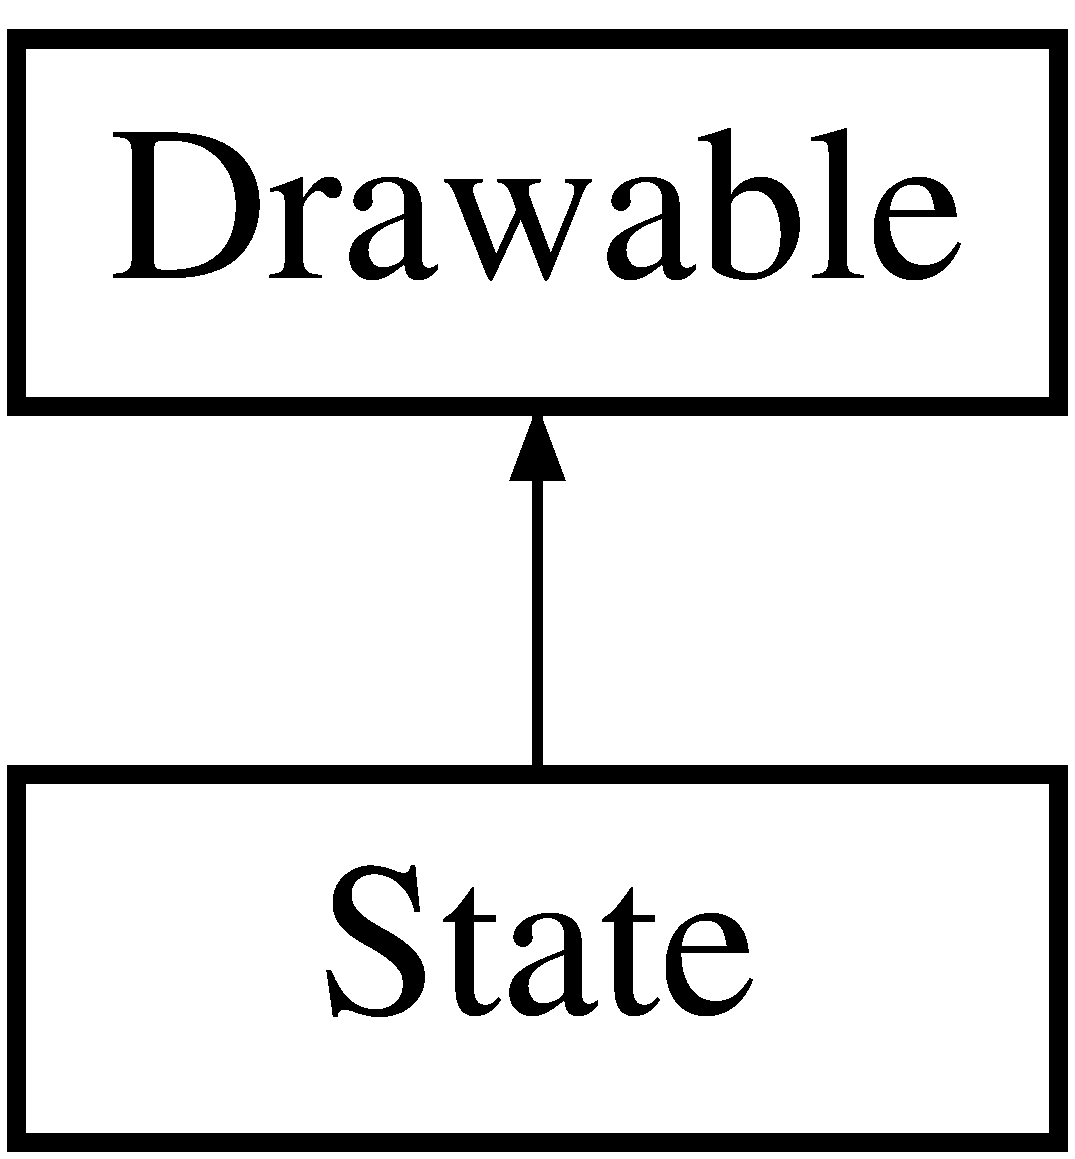
\includegraphics[height=2.000000cm]{class_state}
\end{center}
\end{figure}
\subsection*{Public Member Functions}
\begin{DoxyCompactItemize}
\item 
\mbox{\Hypertarget{class_state_ab91bb1dd5aa6260ab2a456581daf9ec2}\label{class_state_ab91bb1dd5aa6260ab2a456581daf9ec2}} 
\mbox{\hyperlink{class_state_ab91bb1dd5aa6260ab2a456581daf9ec2}{State}} ()
\begin{DoxyCompactList}\small\item\em Default constructor. \end{DoxyCompactList}\item 
\mbox{\Hypertarget{class_state_afab438d92b90dc18d194dbd9c9c8bab3}\label{class_state_afab438d92b90dc18d194dbd9c9c8bab3}} 
virtual \mbox{\hyperlink{class_state_afab438d92b90dc18d194dbd9c9c8bab3}{$\sim$\+State}} ()
\begin{DoxyCompactList}\small\item\em Virtual destructor. \end{DoxyCompactList}\item 
\mbox{\Hypertarget{class_state_a8e83a0c8ff9dd3b0f0fb24f7f1b5b4c4}\label{class_state_a8e83a0c8ff9dd3b0f0fb24f7f1b5b4c4}} 
virtual void \mbox{\hyperlink{class_state_a8e83a0c8ff9dd3b0f0fb24f7f1b5b4c4}{process\+Events}} ()=0
\begin{DoxyCompactList}\small\item\em Process input events for this specific state. \end{DoxyCompactList}\item 
virtual void \mbox{\hyperlink{class_state_acd1d5612d4166c405fb4a11b3a1f1bd3}{update}} (sf\+::\+Time delta\+Time)=0
\begin{DoxyCompactList}\small\item\em Updates the logic for this specific state. \end{DoxyCompactList}\end{DoxyCompactItemize}
\subsection*{Protected Member Functions}
\begin{DoxyCompactItemize}
\item 
virtual void \mbox{\hyperlink{class_state_a7e115388c37a05ee165a395f3119d685}{draw}} (sf\+::\+Render\+Target \&target, sf\+::\+Render\+States states) const =0
\begin{DoxyCompactList}\small\item\em Overrides draw function to draw the current state to the target. \end{DoxyCompactList}\end{DoxyCompactItemize}


\subsection{Detailed Description}
Base class for any screen in the game, including levels. 

\mbox{\hyperlink{class_state}{State}} is a base class for any screen that has input, is updatable, or displayed to the player. You must inherit from this class and add it to the \mbox{\hyperlink{class_state_manager}{State\+Manager}} in your Game derived class in order to access it. 

\subsection{Member Function Documentation}
\mbox{\Hypertarget{class_state_a7e115388c37a05ee165a395f3119d685}\label{class_state_a7e115388c37a05ee165a395f3119d685}} 
\index{State@{State}!draw@{draw}}
\index{draw@{draw}!State@{State}}
\subsubsection{\texorpdfstring{draw()}{draw()}}
{\footnotesize\ttfamily void State\+::draw (\begin{DoxyParamCaption}\item[{sf\+::\+Render\+Target \&}]{target,  }\item[{sf\+::\+Render\+States}]{states }\end{DoxyParamCaption}) const\hspace{0.3cm}{\ttfamily [protected]}, {\ttfamily [pure virtual]}}



Overrides draw function to draw the current state to the target. 


\begin{DoxyParams}{Parameters}
{\em target} & Render target to draw to \\
\hline
{\em states} & Current render states \\
\hline
\end{DoxyParams}
\mbox{\Hypertarget{class_state_acd1d5612d4166c405fb4a11b3a1f1bd3}\label{class_state_acd1d5612d4166c405fb4a11b3a1f1bd3}} 
\index{State@{State}!update@{update}}
\index{update@{update}!State@{State}}
\subsubsection{\texorpdfstring{update()}{update()}}
{\footnotesize\ttfamily void State\+::update (\begin{DoxyParamCaption}\item[{sf\+::\+Time}]{delta\+Time }\end{DoxyParamCaption})\hspace{0.3cm}{\ttfamily [pure virtual]}}



Updates the logic for this specific state. 


\begin{DoxyParams}{Parameters}
{\em delta\+Time} & Time since last update was called \\
\hline
\end{DoxyParams}


The documentation for this class was generated from the following file\+:\begin{DoxyCompactItemize}
\item 
State.\+hpp\end{DoxyCompactItemize}

\hypertarget{class_state_manager}{}\section{State\+Manager Class Reference}
\label{class_state_manager}\index{State\+Manager@{State\+Manager}}


Acts as a wrapper to std\+::stack.  




{\ttfamily \#include $<$State\+Manager.\+hpp$>$}

\subsection*{Public Member Functions}
\begin{DoxyCompactItemize}
\item 
\mbox{\Hypertarget{class_state_manager_a3e2be96d935eb56813b096a885d58587}\label{class_state_manager_a3e2be96d935eb56813b096a885d58587}} 
\mbox{\hyperlink{class_state_manager_a3e2be96d935eb56813b096a885d58587}{State\+Manager}} ()
\begin{DoxyCompactList}\small\item\em Default constructor. \end{DoxyCompactList}\item 
\mbox{\Hypertarget{class_state_manager_a05a43504a033f1befad5c5118249ec6f}\label{class_state_manager_a05a43504a033f1befad5c5118249ec6f}} 
\mbox{\hyperlink{class_state_manager_a05a43504a033f1befad5c5118249ec6f}{$\sim$\+State\+Manager}} ()
\begin{DoxyCompactList}\small\item\em Default destructor. \end{DoxyCompactList}\item 
\mbox{\hyperlink{class_state}{State}} $\ast$ \mbox{\hyperlink{class_state_manager_a76446362726ceb518445e2bdd4814be4}{Current\+State}} ()
\begin{DoxyCompactList}\small\item\em Used to access the current state. \end{DoxyCompactList}\item 
void \mbox{\hyperlink{class_state_manager_a7c6248e6e74dc09736dcc0ed5a622177}{Push\+State}} (\mbox{\hyperlink{class_state}{State}} $\ast$state)
\begin{DoxyCompactList}\small\item\em Adds a \mbox{\hyperlink{class_state}{State}} to the stack. \end{DoxyCompactList}\item 
\mbox{\Hypertarget{class_state_manager_a01cd6f5dafc0add0633b0be231cce665}\label{class_state_manager_a01cd6f5dafc0add0633b0be231cce665}} 
void \mbox{\hyperlink{class_state_manager_a01cd6f5dafc0add0633b0be231cce665}{Pop\+State}} ()
\begin{DoxyCompactList}\small\item\em Removes the \mbox{\hyperlink{class_state}{State}} at the top of the stack. \end{DoxyCompactList}\end{DoxyCompactItemize}


\subsection{Detailed Description}
Acts as a wrapper to std\+::stack. 

\mbox{\hyperlink{class_state_manager}{State\+Manager}} provides an interface to std\+::stack. It has a stack of \mbox{\hyperlink{class_state}{State}} objects and is able to delete them safely on destruction. 

\subsection{Member Function Documentation}
\mbox{\Hypertarget{class_state_manager_a76446362726ceb518445e2bdd4814be4}\label{class_state_manager_a76446362726ceb518445e2bdd4814be4}} 
\index{State\+Manager@{State\+Manager}!Current\+State@{Current\+State}}
\index{Current\+State@{Current\+State}!State\+Manager@{State\+Manager}}
\subsubsection{\texorpdfstring{Current\+State()}{CurrentState()}}
{\footnotesize\ttfamily \mbox{\hyperlink{class_state}{State}} $\ast$ State\+Manager\+::\+Current\+State (\begin{DoxyParamCaption}{ }\end{DoxyParamCaption})}



Used to access the current state. 

\begin{DoxyReturn}{Returns}
A pointer to the current state 
\end{DoxyReturn}
\mbox{\Hypertarget{class_state_manager_a7c6248e6e74dc09736dcc0ed5a622177}\label{class_state_manager_a7c6248e6e74dc09736dcc0ed5a622177}} 
\index{State\+Manager@{State\+Manager}!Push\+State@{Push\+State}}
\index{Push\+State@{Push\+State}!State\+Manager@{State\+Manager}}
\subsubsection{\texorpdfstring{Push\+State()}{PushState()}}
{\footnotesize\ttfamily void State\+Manager\+::\+Push\+State (\begin{DoxyParamCaption}\item[{\mbox{\hyperlink{class_state}{State}} $\ast$}]{state }\end{DoxyParamCaption})}



Adds a \mbox{\hyperlink{class_state}{State}} to the stack. 


\begin{DoxyParams}{Parameters}
{\em state} & Pointer to the \mbox{\hyperlink{class_state}{State}} object to add to the stack \\
\hline
\end{DoxyParams}


The documentation for this class was generated from the following files\+:\begin{DoxyCompactItemize}
\item 
State\+Manager.\+hpp\item 
State\+Manager.\+cpp\end{DoxyCompactItemize}

%--- End generated contents ---

% Index
\backmatter
\newpage
\phantomsection
\clearemptydoublepage
\addcontentsline{toc}{chapter}{Index}
\printindex

\end{document}
